\setcounter{chapter}{3}
\chapter{Implementation}
\minitoc %insert la minitoc
\graphicspath{{Chapitre4/figures/}}

%\DoPToC
%==============================================================================
\pagestyle{fancy}
\fancyhf{}
\fancyhead[R]{\bfseries\rightmark}
\fancyfoot[R]{\thepage}
\renewcommand{\headrulewidth}{0.5pt}
\renewcommand{\footrulewidth}{0pt}
\renewcommand{\chaptermark}[1]{\markboth{{\chaptername~\thechapter. #1 }}{}}
\renewcommand{\sectionmark}[1]{\markright{\thechapter.\thesection~ #1}}

\begin{spacing}{1.2}

%==============================================================================
\section*{Introduction}
This chapter presents the implementation of the LLM-powered best practices enforcement system, detailing how the architectural design from Chapter 3 was translated into a functional system. The implementation encompasses three primary components: the AI agent backend, the IDE extension frontend, and the communication infrastructure that connects them.

The chapter is structured to demonstrate the practical application of the theoretical framework established in previous chapters. It begins with the development environment and infrastructure, then presents the technology stack selections and their rationale, followed by detailed implementation of each system component.

\section{Working Environment}

\subsection{Development Infrastructure}
The implementation leverages Google's internal development infrastructure, providing support for large-scale software development. This infrastructure ensures security, scalability, and integration with existing YouTube development workflows.

\subsubsection{Internal IDE}
The development environment utilizes Google's internal IDE, which provides a development experience similar to Visual Studio Code but optimized for Google's internal infrastructure and security requirements.

\subsubsection{Internal RPC Playground}
The RPC Playground is Google's internal tool for testing and debugging Remote Procedure Call (RPC) services. This tool serves as a playground for sending RPC requests and was essential for developing and testing the communication protocol between the AI Agent and the YouTube IDE Extension.

\subsubsection{Google Colab}
Google Colab was used during early prototyping to iterate on prompt design, tool orchestration, and Executable Agent behaviors before production hardening. Colab provided hosted notebooks with on-demand compute (including GPUs/TPUs) and easy sharing for rapid experiments \cite{colab2017, jupyter2014}. It was part of the development environment rather than the deployed technology stack.

\begin{figure}[H]
    \centering
    
\includegraphics[scale=0.4]{Images/Google_Colab.png}
    \caption{Google Colab Logo}
    \label{fig:google_colab}
\end{figure}

\subsubsection{Internal Repository Integration}
All code is stored and versioned within Google's internal repository system, enabling proper code review processes and collaboration.

\subsection{Project Management and Documentation}

\subsubsection{Internal Version Control}
The project utilizes Google's internal version control system, which provides Git-like functionality while ensuring compliance with internal security and access control requirements. Git is a fast, scalable, distributed version control system designed to handle everything from small to very large projects with speed and efficiency \cite{git2005}.


\subsubsection{Internal Code Review Platform}
Google's internal code review platform provides code review capabilities, ensuring code quality and knowledge sharing across development teams.

The code review platform includes:
\begin{itemize}
    \item \textbf{Automated Review Suggestions}: AI-powered suggestions for code improvements, best practices, and potential issues.
    \item \textbf{Collaborative Review Process}: Tools for managing review workflows, assigning reviewers, and tracking review progress.
    \item \textbf{Integration with CI/CD}: Automatic triggering of builds and tests when code changes are submitted for review.
\end{itemize}

\subsubsection{Internal Project Management System}
The project management system provides project tracking, task management, and collaboration capabilities similar to Jira but optimized for Google's internal workflows. JIRA is a flexible issue tracking system that provides project management capabilities \cite{jira2002}.


\subsubsection{Google Docs}
Google Docs was used for authoring and reviewing design documents, leveraging the internal built-in Approvals workflow to formalize stakeholder sign-off. The review process combined live comments, suggestions, and targeted approvals to ensure traceable decisions.


These project workflows ensured fast iteration, early detection of issues, and compliance with Google's security and code quality standards.



\section{Technologies}

This section presents the concrete technologies used to implement the system. We distinguish between industry-standard tools (e.g., Python, TypeScript, JSON) and internal platforms operated within Google (e.g., YouTube DevInfra Agent Framework, internal AI platform).

\subsection{Backend Technologies (AI Agent)}

\subsubsection{Python Programming Language}
Python serves as the primary programming language for the AI agent framework implementation. Python is a high-level, interpreted programming language known for its simplicity, readability, and library ecosystem \cite{van1995python}. The language's dynamic typing and support for artificial intelligence and machine learning libraries make it suitable for AI agent development \cite{pedregosa2011scikit}.

\begin{figure}[H]
    \centering
    
\includegraphics[scale=0.02]{Images/python_logo.png}
    \caption{Python Programming Language Logo}
    \label{fig:python_logo}
\end{figure}


Python's advantages for this implementation include:
\begin{itemize}
    \item \textbf{AI/ML Ecosystem}: Extensive libraries for machine learning, natural language processing, and AI development.
    \item \textbf{Asynchronous Programming}: Built-in support for asynchronous programming patterns essential for handling concurrent requests.
    \item \textbf{JSON Processing}: Native support for JSON serialization and deserialization required for API communication.
\end{itemize}

% (Colab moved under Development Infrastructure as a prototyping environment)


\subsubsection{YouTube DevInfra Agent Framework}
The implementation utilizes the YouTube DevInfra Agent Framework — the serving infrastructure designed by YouTube for YouTube Developer Infrastructure agents. It underpins all YouTube agents, providing standardized execution, deployment, and operational primitives for LLM-powered applications.

This framework was selected because it natively supports the \textit{Executable Agent} pattern and supplies built-in tool orchestration, workflow control, and production lifecycle management. Using it aligns the implementation with DevInfra standards and avoids rebuilding common agent infrastructure, allowing focus on best-practices enforcement logic.



\subsubsection{Internal AI Platform}
The system integrates with Google's internal AI platform, which hosts internal LLM models trained on Google's codebase, ensuring organization-specific knowledge and compliance with internal security requirements.


\subsubsection{LLM Libraries and Frameworks}
The internal agent framework utilizes several specialized libraries and frameworks for LLM interaction and agent development:

\begin{itemize}
    \item \textbf{LLM Interaction Libraries}: Specialized libraries for communicating with internal LLM models, monitoring token usage, and optimizing API calls.
    \item \textbf{Agent Orchestration Libraries}: Libraries that provide the Executable Agent pattern implementation, tool registration, and workflow management.
    \item \textbf{Prompt Engineering Libraries}: Frameworks for constructing, optimizing, and managing prompts.
\end{itemize}

\subsection{Frontend Technologies (IDE Extension)}

\subsubsection{TypeScript Programming Language}
TypeScript is used for the frontend development of the YouTube IDE Extension. TypeScript is a strongly typed superset of JavaScript that compiles to plain JavaScript \cite{bierman2014understanding}. The language provides static type checking, which helps prevent runtime errors and improves code maintainability in large-scale applications.

TypeScript was chosen because we are building a feature inside an existing extension implemented in TypeScript, ensuring direct compatibility and reuse. Its static typing and interfaces improve maintainability and reduce runtime errors in complex UI state and service interactions. It also integrates seamlessly with VS Code API and other development environments.

\begin{figure}[H]
    \centering
    
\includegraphics[scale=0.05]{Images/Typescript.png}
    \caption{TypeScript Programming Language Logo}
    \label{fig:typescript_logo}
\end{figure}


\subsubsection{VS Code Extension API}
The system integrates with Visual Studio Code through its Extension API. Visual Studio Code is a source-code editor developed by Microsoft, built on the Electron framework \cite{castor2016visual}. The VS Code Extension API provides capabilities for extending the editor's functionality.

Given that the internal IDE is VS Code–like, adopting the VS Code Extension API is the natural choice: it is natively supported within the environment (requiring no additional infrastructure), exposes the command, user‑interface, and configuration interfaces required by the best‑practices enforcement feature, and ensures compatibility with the existing extension ecosystem. In practice, the API provides the integration points necessary to implement the designed interaction flow without introducing custom runtime scaffolding.


\subsubsection{JSON Data Format}
JSON (JavaScript Object Notation) is used for data serialization and configuration management throughout the system. JSON is a lightweight, text-based data interchange format that is easy for humans to read and write \cite{crockford2006application}.

JSON was chosen because the agent returns a string payload over RPC; encoding structured results as JSON preserves human readability and cross-language compatibility while satisfying the transport constraint.

Compared to gRPC with Protocol Buffers, JSON trades schema rigor and compact binary encoding for human‑readability and ease of inspection. This project prioritizes operability within the IDE and debuggability during development, so JSON was preferred, with explicit schema validation applied at boundaries to mitigate the lack of strong compile‑time contracts.



\section{Realization}

\subsection{Agent Implementation}
The AI Agent implementation follows the Executable Agent architecture pattern established in Chapter 3, providing deterministic execution with reliability and performance compared to alternative approaches. The implementation leverages Python's AI/ML ecosystem and Google's internal AI platform to create a scalable solution for YouTube framework best practices enforcement.

% (Removed redundant Development Environment Setup; infrastructure and repositories are covered in Working Environment)

\subsubsection{Agent Configuration and Initialization}
The agent initialization process involves several critical configuration steps that ensure proper operation within the Google infrastructure:

\begin{itemize}
    \item \textbf{Model Selection}: The agent is configured to use the latest internal Gemini-based model, specifically trained on Google's codebase.
    \item \textbf{Convention Loading}: At startup, the agent loads YouTube framework best practices from JSON configuration files stored in the internal repository.
    \item \textbf{Tool Registration}: All five specialized tools are registered with the agent framework, establishing the deterministic workflow pattern.
    \item \textbf{Error Handling Setup}: Comprehensive error handling mechanisms are initialized, including retry policies, timeout configurations, and fallback strategies.
\end{itemize}


\paragraph{Implementation Structure}
The agent is implemented as a class that exposes a single execute entry point responsible for orchestrating analysis. Tools are implemented as separate classes that expose a run method and encapsulate focused responsibilities (e.g., prompt construction, model invocation, response parsing). Public contracts specify inputs, outputs, and typed errors for each tool, while the agent coordinates them via a registry and passes dependency‑injected helpers and shared utilities. Each tool also records token usage per invocation and emits lightweight metrics for observability. This class‑based structure improves testability (mockable tool interfaces), maintainability (clear separation of concerns), and extensibility (tools can be replaced or added without modifying the orchestration logic).
\subsubsection{Core Tools Implementation}
The agent implements five specialized tools, each handling a specific aspect of the best practices analysis pipeline as defined in Chapter 3:

\paragraph{ReadFileFromWorkspace Tool}
Design contract: input = file path; output = full file content.
The ReadFileFromWorkspace tool handles file system access and content retrieval operations. This tool implements error handling for common file system issues, including file not found errors, permission violations, and encoding problems. The tool handles multiple file formats and encodings that might arise in different development environments, providing error reporting to facilitate debugging and user feedback.

\paragraph{CodeAnalysisTool}
Design contract: input = file content; output = list of base violations.
The CodeAnalysisTool serves as the core analysis engine, performing code analysis using LLM capabilities. The tool implements prompt engineering techniques to ensure consistent and accurate analysis results. The prompt construction process incorporates context-aware information, including file type, and relevant convention definitions.

\subparagraph{Prompt Engineering Implementation}
The CodeAnalysisTool implements a multi-stage prompt construction process that ensures optimal LLM performance:

\begin{itemize}
    \item \textbf{Context Injection}: The tool dynamically injects relevant YouTube framework conventions based on file type and detected patterns, ensuring that the LLM has access to the most relevant best practices.
    \item \textbf{Template System}: A template system allows for consistent prompt formatting while accommodating different file types and analysis contexts.
\end{itemize}

% (Removed temperature tuning details to reflect implemented scope)

\subparagraph{Performance Notes}
Selected optimizations implemented:

\begin{itemize}
    \item \textbf{Caching Mechanism}: Convention definitions and prompt templates are cached in memory to reduce repeated processing overhead.
    \item \textbf{Response Parsing}: JSON parsing with error recovery ensures handling of LLM responses.
\end{itemize}

\paragraph{ViolationExplanationTool}
Design contract: input = base violation; output = natural-language explanation.
The ViolationExplanationTool generates human-readable explanations for identified violations. This tool implements natural language generation techniques to provide clear, educational explanations that help developers understand not only what violations exist, but why they are problematic and how they impact code quality.

The explanation generation process incorporates contextual information about the violation, surrounding code, and relevant best practices. This contextual approach ensures that explanations are specific, relevant, and actionable for developers.

\paragraph{CodeFixTool}
Design contract: input = base violation + explanation; output = suggested fix.
The CodeFixTool provides actionable fix suggestions for identified violations. The tool implements code generation techniques that produce fixes designed to be:
\begin{itemize}
    \item \textbf{Safe}: Only modify internal implementation without breaking public APIs
    \item \textbf{Self-contained}: Require no additional changes in other files
    \item \textbf{Contextual}: Take into account the specific code context and framework patterns
    \item \textbf{Educational}: Include comments explaining the reasoning behind the fix
\end{itemize}
The generated fixes include explanatory comments to help developers understand the reasoning behind the suggested changes.

The fix generation process prioritizes safety and correctness, ensuring that suggested changes maintain the original functionality while addressing the identified violations. The tool also considers the broader codebase context to ensure that fixes align with existing patterns and conventions.

\paragraph{Finish Tool}
Design contract: input = violation results + explanations + fixes; output = structured response format.
The Finish tool serves as the consolidation component, aggregating all analysis results into a structured output format. This tool implements result validation, ensuring that the output contains all necessary information for the IDE extension to display results effectively.

The consolidation process includes deduplication of overlapping violations, merging of related issues, and formatting of results for optimal presentation.


\subsubsection{Processing Strategy Architecture}
The agent implements the hybrid parallel processing strategy with concurrency limiting as described in Chapter 3. This approach balances the benefits of concurrent processing with the need for system stability and resource management. The implementation uses \textbf{semaphore-based concurrency control} to limit the number of concurrent LLM calls, preventing resource saturation while maintaining optimal performance.

The internal workflow is illustrated in the activity diagram below:

\begin{figure}[H]
	\centering
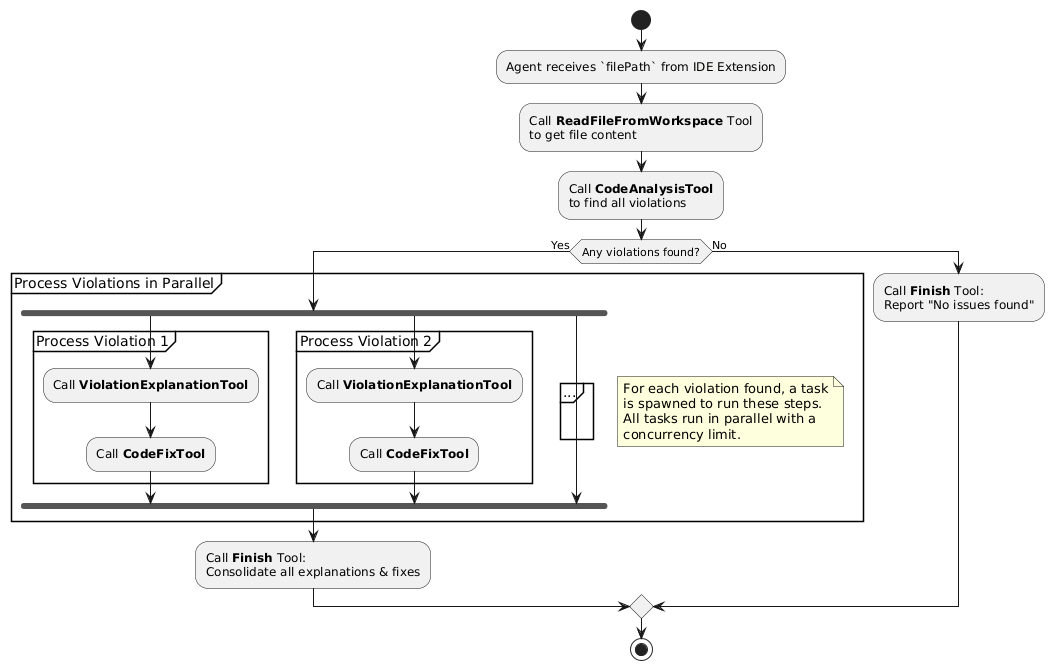
\includegraphics[scale=0.5]{images/activity_diagram.png}
\caption{Agent Processing Activity Diagram}
\label{fig:agent_activity}
\end{figure}

This activity diagram illustrates the hybrid processing strategy in action, showing how the agent balances sequential and parallel processing to optimize performance and reliability.

This workflow represents the processing scenario that occurs when the agent analyzes a file with multiple violations.

\paragraph{Sequential Initial Processing}
The agent begins with sequential steps to ensure that the complete code context is available before any analysis begins, and all violations are identified before parallel processing starts.

\paragraph{Parallel Violation Processing}
When violations are found, the agent employs the hybrid processing strategy. Each violation is processed independently, with explanation generation and fix creation happening concurrently across multiple violations while maintaining system stability.

\paragraph{Result Consolidation}
The workflow concludes with result consolidation, ensuring that all processing results are properly aggregated into a coherent response format for the YouTube IDE Extension.

\paragraph{Concurrency Control Implementation}
The implementation uses a semaphore-based concurrency control system with concurrency limiting to limit the number of concurrent LLM calls. A default concurrency limit is applied per worker pool, and excess tasks are queued in a FIFO (First In, First Out) queue to prevent resource saturation. This ensures that the system remains stable even under high load conditions.

\subsubsection{Error Handling and Resilience}
The system implements error isolation mechanisms where failures in one violation processing task do not stop the processing of other violations. Each violation is processed independently, and partial results are persisted even when individual tasks fail. This approach ensures that developers receive feedback even when some analysis steps encounter errors.

The implementation includes retry mechanisms with exponential backoff for transient failures, ensuring operation in production environments. The error handling system implements specific error types for different failure scenarios, including file system errors, network communication errors, LLM processing errors, and agent orchestration errors. Each error type includes detailed error information and suggested recovery actions to facilitate debugging and user support.

\subsubsection{Convention Data Management}
The convention data management system implements loading, caching, and retrieval mechanisms for YouTube framework best practices. The conventions are stored as Python objects in an array, each containing a unique identifier, description, correct example, and incorrect example. For efficient runtime access, the system constructs an in-memory map keyed by convention ID, allowing the agent tools to retrieve only the relevant convention on demand. 

\paragraph{Loading and Initialization}
At startup, all convention objects are loaded into memory from the Python array. A dictionary (map) is created with convention IDs as keys and convention objects as values, providing constant-time access for subsequent tool invocations.

\paragraph{Memory Caching and Access}
This in-memory caching strategy ensures low-latency access during code analysis:

\begin{itemize}
    \item \textbf{Efficient Lookup}: Tools retrieve conventions by ID from the map, avoiding iteration over the full array.
    \item \textbf{Dynamic Selection}: Only conventions relevant to the current file type and analysis context are queried, minimizing unnecessary data processing.
    \item \textbf{Lightweight and Fast}: The cache resides entirely in memory, requiring no external services, and supports rapid retrieval during concurrent tool executions.
\end{itemize}


\subsection{Extension Integration}

\subsubsection{Extension Architecture}
The IDE Extension implements a layered architecture that integrates with the overall system through three distinct layers: the Extension layer containing user-facing components, a Proxy layer for authentication and request routing, and the Backend layer hosting AI agent services.

\begin{figure}[H]
    \centering
    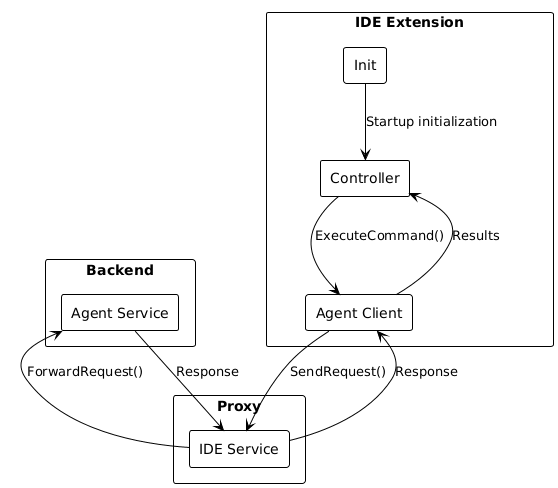
\includegraphics[scale=0.6]{Images/extension_integration.png}
    \caption{System Architecture: IDE Extension, Proxy, and Backend Communication Flow}
    \label{fig:high_level_frontend_architecture}
\end{figure}

The architecture follows a clear request-response pattern where user interactions trigger analysis requests that flow through the IDE Service proxy for authentication and authorization, then to the Agent Service in the backend for processing. Responses follow the same path in reverse, ensuring secure and authenticated communication throughout the entire pipeline while maintaining clear separation of responsibilities between layers.

\subsubsection{Extension Components}
The extension's internal architecture consists of three core components that work together to provide seamless integration with the development environment, as illustrated in Figure~\ref{fig:high_level_frontend_architecture}.

\textbf{Init Component}: Handles extension initialization, reading user settings, registering commands and editor actions, and performing health checks. The component ensures proper setup of all dependencies.

\textbf{Controller}: Centralizes all UI-related state and orchestrates interactions between components. The Controller processes commands, manages notifications, routes analysis results, renders diagnostics and hover-based suggestions, and coordinates stale-state transitions to ensure consistent behavior across all entry points.

\textbf{AgentClient}: Manages communication with the backend services through the proxy layer. The component handles request formatting, implements retry logic with exponential backoff, manages timeouts, and processes responses from the AI agent.

\subsubsection{User Interaction}
The feature is controlled through a dedicated \textbf{user setting}. This setting appears as a simple checkbox: when enabled, the feature becomes available in the IDE; when disabled, it is entirely hidden from the interface. This ensures that developers can opt in seamlessly without cluttering the environment for those who do not use the feature.

The primary entry point for triggering analysis is an \textbf{Editor Action} integrated into the file title bar (Figure~\ref{fig:editor_action_implementation}). This placement ensures high visibility and aligns naturally with the developer’s workflow when working on individual files.

\begin{figure}[H]
    \centering
    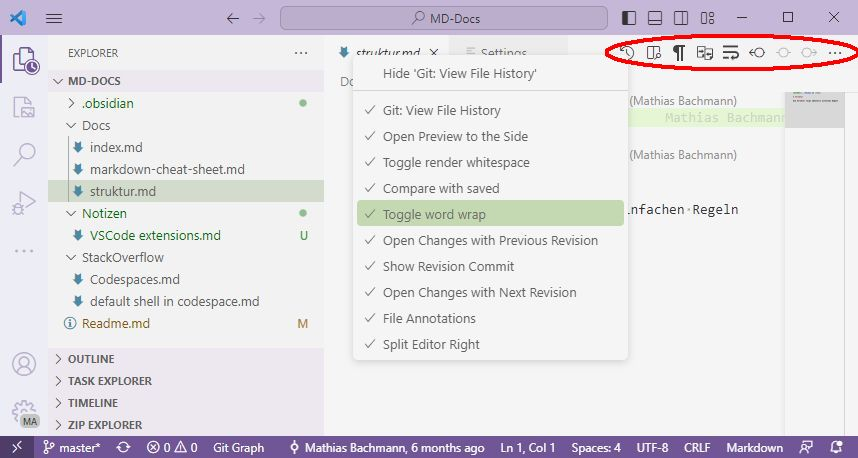
\includegraphics[scale=0.4]{Images/editor_actions.jpg}
    \caption{VS Code Interface: Editor Actions (Illustrative).}
    \label{fig:editor_action_implementation}
\end{figure}

An additional entry point is provided through the \textbf{Command Palette}, which can be invoked using \texttt{Ctrl+Shift+P} (or \texttt{Cmd+Shift+P} on macOS). This pathway makes the feature equally accessible to developers who prefer keyboard-driven workflows and ensures discoverability for new users exploring available commands (Figure~\ref{fig:command_palette_example}).

\begin{figure}[H]
    \centering
    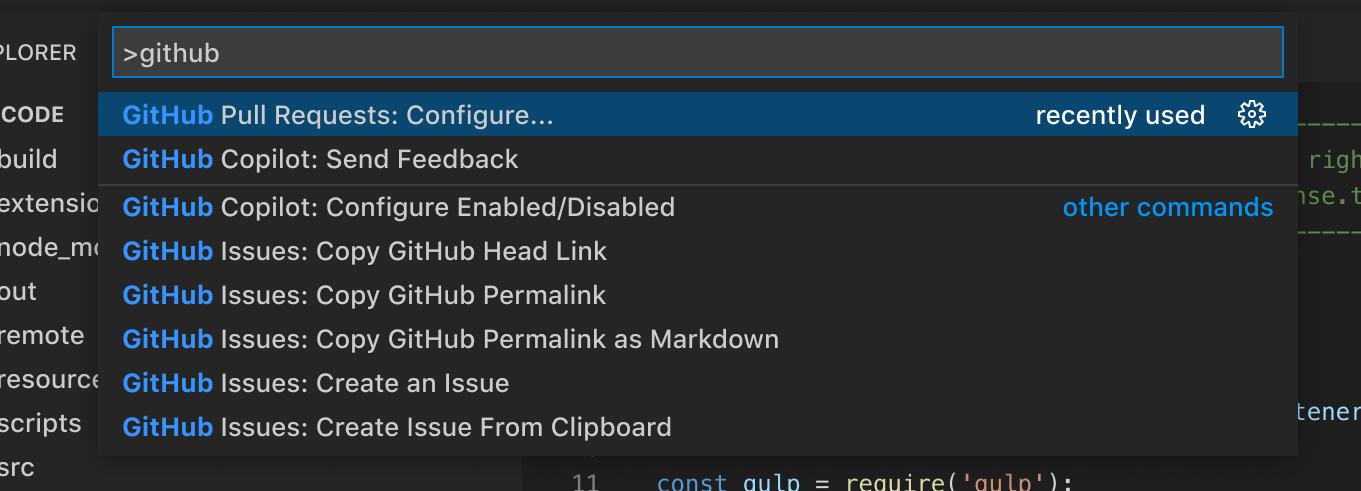
\includegraphics[scale=0.5]{Images/command_palette.png}
    \caption{VS Code Command Palette (Illustrative).}
    \label{fig:command_palette_example}
\end{figure}


Once analysis is triggered, the extension provides immediate feedback via \textbf{VS Code notifications} (Figure~\ref{fig:notification_example}). These notifications confirm that a request has been received, update progress, and display clear error messages if issues occur. This ensures transparent communication throughout the request lifecycle.

\begin{figure}[H]
    \centering
    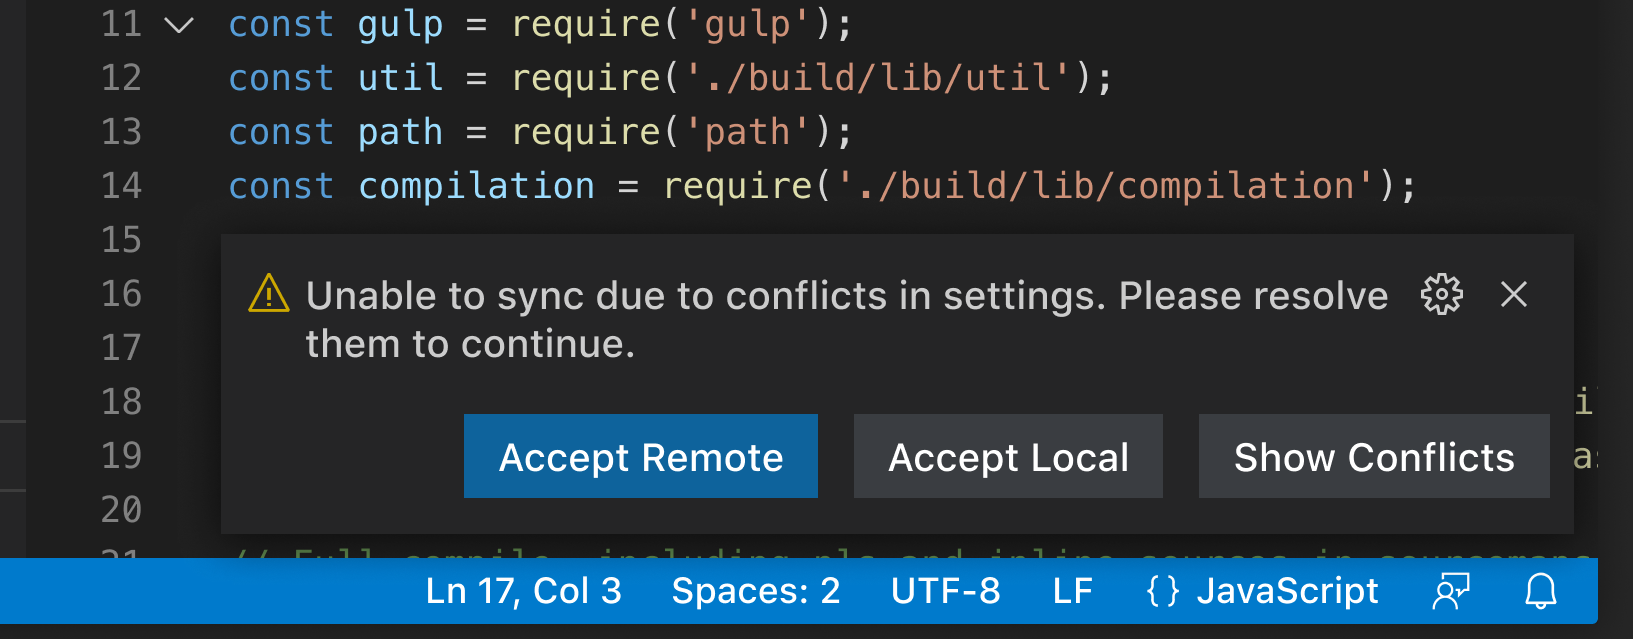
\includegraphics[scale=0.8]{Images/vscode_notification.png}
    \caption{VS Code Notification Interface (Illustrative).}
    \label{fig:notification_example}
\end{figure}

The results of the analysis are surfaced through VS Code’s native \textbf{diagnostic system}. Violations appear in the \textbf{Problems panel} and are underlined directly in the editor, marking the exact range of code that violates a best practice (Figure~\ref{fig:diagnostics_example}). Hovering over the highlighted code reveals the diagnostic explanation, helping developers quickly understand the issue in context.

\begin{figure}[H]
    \centering
    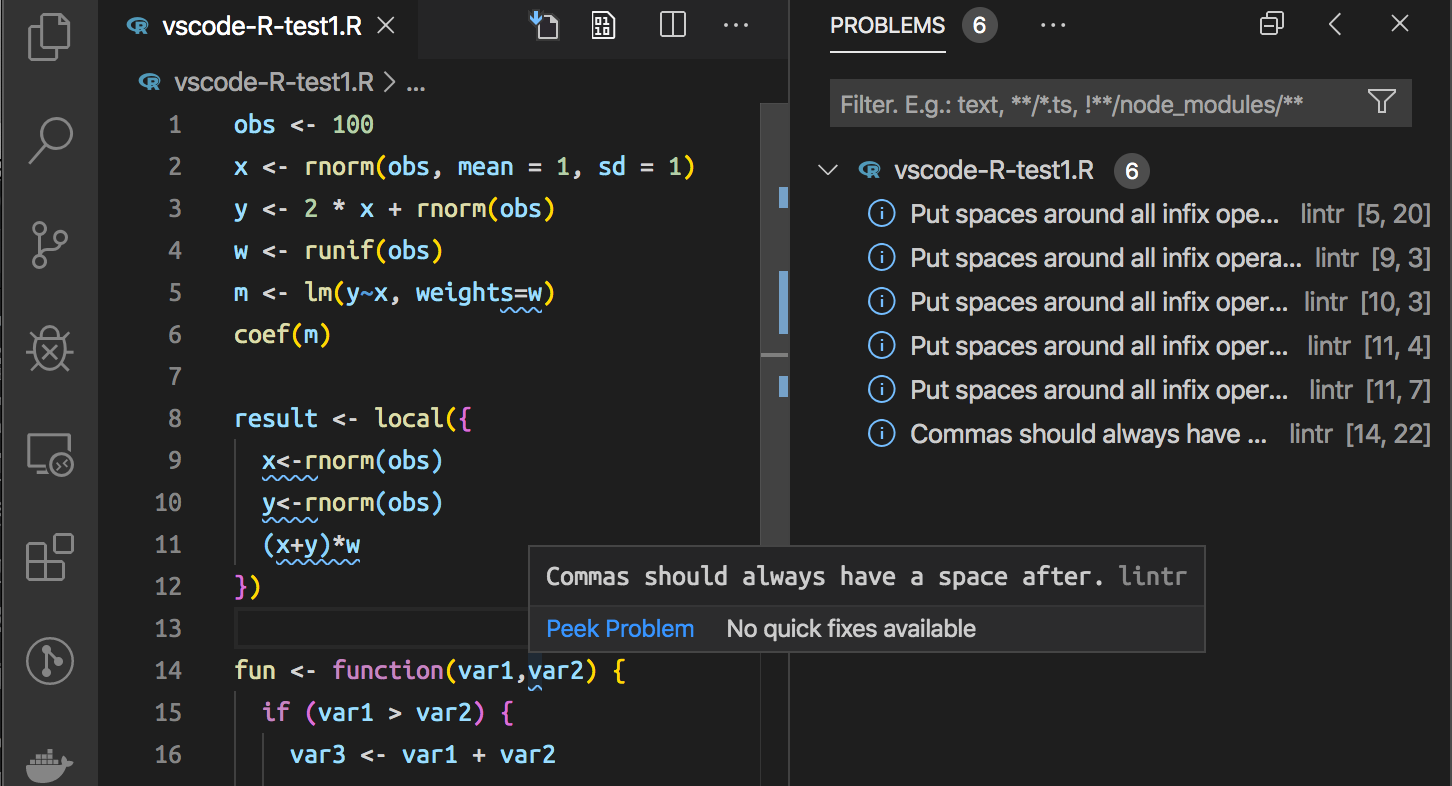
\includegraphics[scale=0.4]{Images/vscode_diagnostics.png}
    \caption{VS Code Diagnostics Interface (Illustrative).}
    \label{fig:diagnostics_example}
\end{figure}

For more detailed guidance, an integrated \textbf{hover provider} presents formatted fix suggestions directly within the editor. This approach allows fixes to be displayed with proper syntax highlighting and inline code snippets, offering a clear and actionable path to resolution without leaving the development workflow.

\subsubsection{Stale Diagnostics Handling}
One of the most challenging aspects of IDE integration is maintaining diagnostic accuracy as developers continuously modify their code. The extension implements a sophisticated two-tiered system that balances immediate responsiveness with accurate analysis results.

\paragraph{The Challenge}
Traditional diagnostic systems struggle with code that changes rapidly, often displaying outdated information that confuses developers and reduces trust in the tool. The challenge is to provide immediate visual feedback while ensuring that diagnostics remain accurate and relevant to the current code state.

\paragraph{Two-Tiered Solution}  
The extension handles stale diagnostics using a two-tiered approach that separates immediate responsiveness from precise re-anchoring:  

\textbf{Tier 1 - Instant Adjustment}: Provides immediate feedback on every keystroke. Diagnostics are shifted based on simple text edits and marked as [Outdated] if the flagged code itself is edited. This ensures high \textbf{responsiveness} without impacting performance.  

\textbf{Tier 2 - Debounced Re-anchoring}: Activates after a 1-second pause in typing to improve diagnostic \textbf{accuracy}. The process involves:  
\begin{enumerate}
    \item \textbf{Fingerprint}: Creates a contextual hash from the code and its surrounding context to identify exact matches.  
    \item \textbf{Scan with Regex}: Finds all possible text matches across the document.  
    \item \textbf{Re-anchor}: Moves the diagnostic to the correct new location based on the highest match score.  
\end{enumerate}  
This two-tiered strategy balances responsiveness with accuracy, ensuring developers receive timely feedback while maintaining the integrity of diagnostics even during active code editing.


\begin{figure}[H]
    \centering
    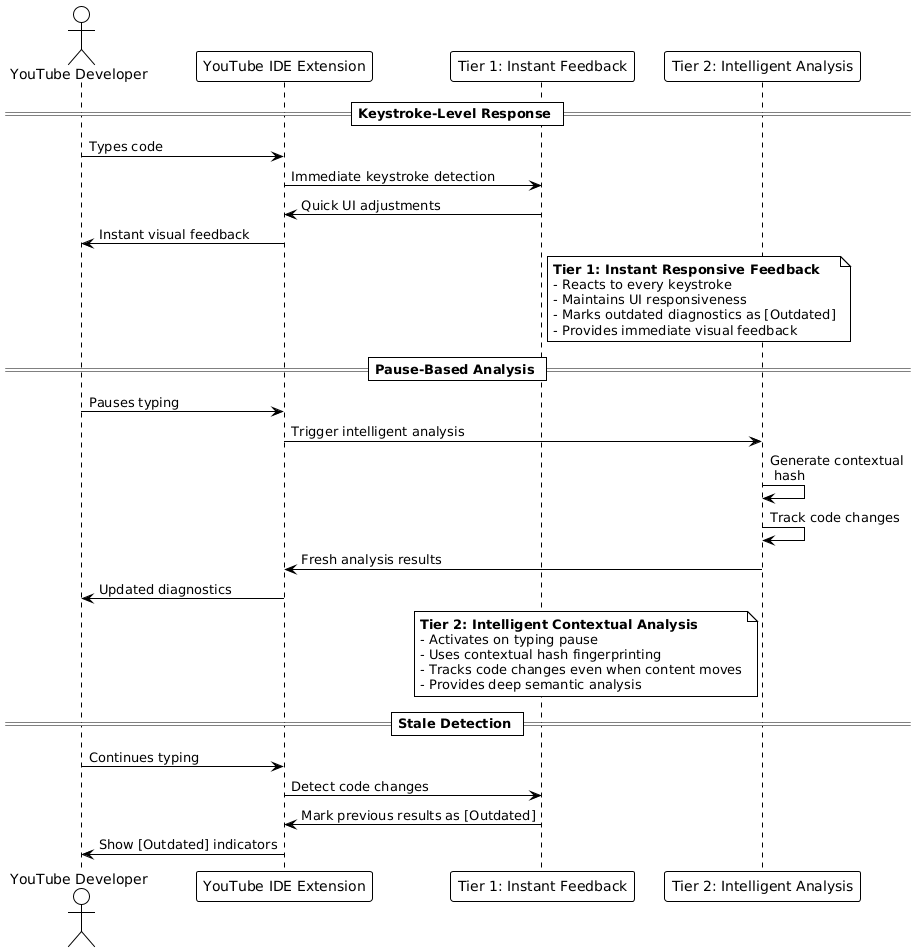
\includegraphics[scale=0.6]{Images/stale_diagnostics.png}
    \caption{Stale Diagnostics Handling: Two-Tiered System (Illustrative)}
    \label{fig:stale_diagnostics_method}
\end{figure}

This approach ensures that developers receive immediate visual feedback while maintaining diagnostic accuracy through intelligent analysis timing and state management, representing a significant technical contribution to IDE integration challenges.

\subsubsection{Resilience and Communication}
The extension implements comprehensive error handling and resilience mechanisms to ensure reliable operation in production environments. The communication system uses internal RPC infrastructure with JSON payloads for debugging and cross-language compatibility.

Error handling follows fault-tolerant design principles with multi-level error isolation, ensuring that failures in one component do not cascade to others. The system implements specific error types for different failure scenarios, including network communication errors, service unavailability, and timeout errors, with detailed error information and suggested recovery actions.

Retry mechanisms with exponential backoff and bounded attempts ensure operation under transient failure conditions, while timeout management prevents indefinite waiting periods and maintains responsive user experience. The implementation includes request validation and response parsing to prevent communication errors and ensure data integrity throughout the analysis pipeline.


\section*{Conclusion}
This chapter presented the implementation of the LLM-powered best practices enforcement system, detailing the development environment, technology stack, and practical realization. The implementation successfully translates the architectural design from Chapter 3 into a functional system that integrates AI agent capabilities with IDE extension functionality.

The implementation establishes a solid foundation for real-world deployment and future enhancements, setting the stage for the performance evaluation presented in Chapter 5.

%==============================================================================
\end{spacing}